\documentclass[a4paper,13pt]{article} % Tạo một bản báo cáo
\usepackage[utf8]{inputenc}
\usepackage[T5]{fontenc} % Để sử dụng tiếng Việt
\usepackage[fontsize=13pt]{scrextend} 
\usepackage[paperheight=29.7cm, paperwidth=21cm, right=20mm,left=30mm,top=25mm,bottom=25mm]{geometry} % Chuẩn A4, căn lề phải, trái, trên, dưới
\usepackage{biblatex}
\addbibresource{references.bib} % File .bib chứa thông tin tham khảo
\usepackage{mathptmx} % Time New Roman
\usepackage{graphicx} % Thư viện chèn ảnh
\usepackage{float} % Set vị trí chèn ảnh
\usepackage{tikz} % Thư viện tạo khung bìa
\usetikzlibrary{calc} % Thư viện tikz
\usepackage{xcolor} % Sử dụng màu sắc
\usepackage{colortbl} % Tô màu cho bảng
\usepackage{array} % Tạo bảng
\usepackage{lettrine} % chữ đầu to
\usepackage{multicol} % Gói để tạo nhiều cột
\usepackage{tocloft} % Gói tùy chỉnh mục lục
\usepackage{booktabs}  
\usepackage[labelformat=empty]{caption}
\usepackage{hyperref} % Tạo liên kết trong mục lục
\usepackage{bookmark} % Cải thiện bookmark
\usepackage{titletoc}
\usepackage{amsmath}
\usepackage{fancyhdr}
\pagestyle{fancy}
\usepackage{utopia}
\renewcommand*{\bibfont}{\small}
\renewcommand{\thesection}{\Roman{section}}

% Tạo header
\fancyhf{}
\chead{\textbf{\textit{Công nghệ tần số mới mmWave, THz Communication}}}
\lfoot{\textbf{\textit{SVTH: Nguyễn Bá Thành \hspace{2cm} Hướng dẫn: PGS.Lê Thị Phương Mai}}}
\rfoot{\thepage}
\renewcommand{\headrulewidth}{1pt}
\renewcommand{\footrulewidth}{1pt}


\thispagestyle{empty}

% Tùy chỉnh mục lục bảng và hình ảnh
\renewcommand{\cftsubsecpresnum}{}
\renewcommand{\listfigurename}{}
\renewcommand{\listtablename}{}

% Tùy chỉnh định dạng mục lục hình ảnh và bảng
\renewcommand{\cftfigpresnum}{Hình }
\renewcommand{\cftfigaftersnum}{: }
\setlength{\cftfignumwidth}{1cm}

\renewcommand{\cfttabpresnum}{Bảng }
\renewcommand{\cfttabaftersnum}{: }
\setlength{\cfttabnumwidth}{1cm}


\begin{document}
\renewcommand{\thesection}{}
\renewcommand{\thesubsection}{}
\begin{titlepage}
\begin{tikzpicture}[overlay,remember picture]
\draw [line width=3pt]
($ (current page.north west) + (2.5cm, -1.5cm) $)
rectangle
($ (current page.south east) + (-1.5cm, 1.5cm) $);
\draw [line width=0.5pt]
($ (current page.north west) + (2.4cm, -1.6cm) $)
rectangle
($ (current page.south east) + (-1.4cm, 1.6cm) $);
\end{tikzpicture}

\begin{center}
\vspace{-6pt}
\textbf{\fontsize{18pt}{0pt}\selectfont ĐẠI HỌC ĐÀ NẴNG} \\
\textbf{\fontsize{18pt}{0pt}\selectfont TRƯỜNG ĐẠI HỌC BÁCH KHOA} \\
\textbf{\fontsize{18pt}{0pt}\selectfont KHOA ĐIỆN TỬ - VIỄN THÔNG}
\end{center}

\begin{center}
\begin{figure}[H]
    \centering
    
\includegraphics[scale=0.5]{logo.jpg} % Giảm kích thước ảnh xuống 50%
    \label{fig:logo_scale}
\end{figure}
\end{center}

\begin{center}
\textbf{\fontsize{30pt}{0pt}\selectfont BÁO CÁO CUỐI KÌ}  \\ 
\vspace{15pt}
\textbf{\fontsize{17pt}{0pt}\selectfont MÔN HỌC: Mạng và hệ thống truyền thông tiên tiến} \\
\vspace{30pt}
\textbf{\fontsize{15pt}{0pt}\selectfont ĐỀ TÀI:} \\ 
\vspace{15pt}
\fontsize{20pt}{0pt}\selectfont Công nghệ tần số mới mmWave, THz Comunication
\end{center}
\vspace{40pt}

\begin{flushleft}
\hspace{4cm}Sinh viên thực hiện \hspace{0.05cm}: Nguyễn Bá Thành \\
\hspace{4cm}Lớp \hspace{3.2cm}: 21DTCLC4 \\
\hspace{4cm}Nhóm \hspace{2.7cm}: 21.40 \\
\hspace{4cm}MSSV \hspace{2.7cm}: 106210200 \\
\hspace{4cm}Giảng viên \hspace{1.8cm}: PGS.TS.Lê Thị Phương Mai \\
\end{flushleft}
\vspace{3cm}
\begin{center}
    \textit{Tháng 5 năm 2025}
\end{center}
\end{titlepage}

\begin{center}
\section{TÓM TẮT}
\end{center}
Tên đề tài: Công nghệ tần số mới mmWave, THz Communication \\
Sinh viên thực hiện: Nguyễn Bá Thành\\
Số thẻ SV: 106210200 Lớp: 21.40 \\

mmWave, THz hiểu đơn giản là gì ? Điều gì khiến chúng trở nên đặc biệt ? Bài viết này sẽ giới thiệu cho bạn những điều cơ bản về sóng milimet, bao gồm định nghĩa, công nghệ cốt lõi, hạn chế và ưu điểm của chúng.

Công nghệ mmWave (sóng milimet), hoạt động trong dải tần 30-300 GHz, là một trụ cột quan trọng của mạng 5G, mang lại tốc độ truyền dữ liệu cực cao và độ trễ thấp. Hiện nay, nhiều quốc gia đã triển khai mmWave trong các khu vực đô thị để phục vụ các ứng dụng tiên tiến như thực tế ảo (VR), y tế từ xa và cảm biến thông minh. Các quốc gia dẫn đầu bao gồm: \\
\begin{itemize}
    \item Hoa Kỳ: Các nhà mạng như Verizon và AT&T đã triển khai mmWave ở các thành phố lớn như New York và Los Angeles.
    \item Trung Quốc: China Mobile và Huawei đang đẩy mạnh ứng dụng mmWave trong các đô thị lớn như Bắc Kinh và Thượng Hải.
    \item Nhật Bản: SoftBank và NTT Docomo sử dụng mmWave để hỗ trợ mạng 5G tốc độ cao.
    \item Châu Âu: Các nước như Đức, Ý và Phần Lan cũng đang thử nghiệm và triển khai mmWave.
\end{itemize}
Ví dụ, Qualcomm từng ghi nhận tốc độ tải xuống 4,3 Gbps trong thử nghiệm mmWave vào năm 2020, minh họa tiềm năng vượt trội của công nghệ này. Trong khi đó, THz (teraherz), với dải tần 0.1-10 THz, vẫn đang trong giai đoạn nghiên cứu nhưng hứa hẹn tốc độ dữ liệu lên đến hàng trăm Gbps, vượt xa mmWave. Các nước như Hoa Kỳ, Nhật Bản và Trung Quốc đang đầu tư mạnh vào nghiên cứu THz tại các viện nghiên cứu và trường đại học.\\

Tại Việt Nam, mmWave đang được các nhà mạng lớn như Viettel, VNPT và MobiFone tích hợp vào mạng 5G, tập trung ở các thành phố lớn như Hà Nội và TP. Hồ Chí Minh. Ví dụ, Viettel đã bắt đầu thử nghiệm 5G sử dụng mmWave từ năm 2020, với mục tiêu phủ sóng các khu vực đông dân cư. Trong khi đó, THz vẫn ở giai đoạn nghiên cứu ban đầu, chủ yếu tại các cơ sở học thuật như Đại học Bách Khoa Hà Nội và Viện Hàn lâm Khoa học và Công nghệ Việt Nam.
\vspace{2cm}
\clearpage  
\begin{center}
\section{LỜI NÓI ĐẦU VÀ CẢM ƠN }
\end{center}

Trong những thập kỷ gần đây, Việt Nam đang trải qua một kỷ nguyên phục hưng công nghệ đầy ấn tượng, từng bước khẳng định vị thế của mình trên bản đồ công nghệ toàn cầu. Từ một quốc gia vốn chủ yếu dựa vào nông nghiệp, Việt Nam đã chuyển mình để trở thành một trung tâm công nghệ sôi động, đạt được những bước tiến vượt bậc trong các lĩnh vực như viễn thông, công nghệ thông tin và các công nghệ tiên tiến mới nổi. Trong số đó, công nghệ tần số cao như mmWave (sóng milimet) và THz (Terahertz) đang nổi lên như một hướng đi đầy tiềm năng, hứa hẹn mang lại những thay đổi đột phá cho tương lai.\\

Công nghệ mmWave và THz nổi bật với khả năng cung cấp băng thông cực rộng, tốc độ truyền dữ liệu siêu nhanh và hỗ trợ kết nối cho hàng tỷ thiết bị trong hệ sinh thái IoT (Internet of Things). Những đặc tính này không chỉ mở ra cơ hội cho các ứng dụng viễn thông thế hệ mới mà còn thúc đẩy sự phát triển của nhiều lĩnh vực công nghệ tiên tiến khác. Tại Việt Nam, các doanh nghiệp hàng đầu như VNPT, Viettel và FPT đang tích cực đầu tư nghiên cứu và triển khai các giải pháp dựa trên hai công nghệ này, với mục tiêu đưa Việt Nam trở thành một trung tâm công nghệ tiên phong trong khu vực Đông Nam Á.\\

Trong bối cảnh đó, Trường Bách khoa Đà Nẵng, một trong những cơ sở giáo dục kỹ thuật hàng đầu của Việt Nam, đang đóng vai trò quan trọng trong việc đào tạo nguồn nhân lực chất lượng cao và thúc đẩy nghiên cứu về công nghệ tần số cao. Với các chương trình đào tạo tiên tiến và các dự án nghiên cứu mang tính đột phá, nhà trường không chỉ góp phần nâng cao năng lực công nghệ quốc gia mà còn trực tiếp tham gia vào sự phát triển của mmWave và THz tại Việt Nam. Đây là minh chứng cho cam kết của trường trong việc đồng hành cùng kỷ nguyên phục hưng công nghệ của đất nước.\\

Đặc biệt, cô Lê Thị Phương Mai, một giảng viên và nhà nghiên cứu tại Trường Bách khoa Đà Nẵng, đã có những đóng góp nổi bật trong lĩnh vực này. Với vai trò là người hướng dẫn và tham gia các dự án nghiên cứu liên quan đến mmWave và THz, cô không chỉ góp phần nâng cao hiểu biết mà còn thúc đẩy ứng dụng thực tiễn của các công nghệ này tại Việt Nam. Những nỗ lực của cô và đội ngũ tại Trường Bách khoa Đà Nẵng đang tạo nên nền tảng vững chắc để Việt Nam tiến xa hơn trong lĩnh vực công nghệ tần số cao.\\

Nhìn chung, với sự kết hợp giữa các doanh nghiệp công nghệ hàng đầu, các viện nghiên cứu và những cơ sở giáo dục xuất sắc như Trường Bách khoa Đà Nẵng, Việt Nam đang vững bước trên con đường trở thành một cường quốc công nghệ trong tương lai gần. Công nghệ mmWave và THz không chỉ là một phần quan trọng của hành trình này mà còn là biểu tượng cho những cơ hội và triển vọng rộng mở, đưa Việt Nam vươn lên mạnh mẽ trong kỷ nguyên phục hưng công nghệ toàn cầu.
\clearpage  

\begin{center}
\section{MỤC LỤC}
\end{center}

\renewcommand{\contentsname}{}
\tableofcontents % Tạo mục lục
\clearpage

\begin{center}
\section{DANH MỤC HÌNH ẢNH, BẢNG BIỂU}
\end{center}
\listoffigures
\clearpage


\section{Chương 1: Tình hình hiện nay của mmWave và THz}
Hình tròn màu xanh biểu thị 4G với tốc độ khoảng 10-100 Mbps. Đây là thế hệ mạng đầu tiên hỗ trợ truyền dữ liệu tốc độ cao cho điện thoại thông minh sử dụng dải tần Sub-6GHz \\
Hình tròn màu tím biểu thị 5G với tốc độ khoảng 0,1-1 Gbps đánh dấu bước nhảy vọt nhờ sử dụng dải tần mmWave, hỗ trợ ứng dụng như video 4K và IOT \\
Hình tròn màu hồng biểu thị 6G với tốc độ chưa được xác định, dự kiến sử dụng dải tần THz 100-300 GHz với mục tiêu hỗ trợ các dự án về AI, xe tự hành
\begin{figure}[htbp]
    \centering
    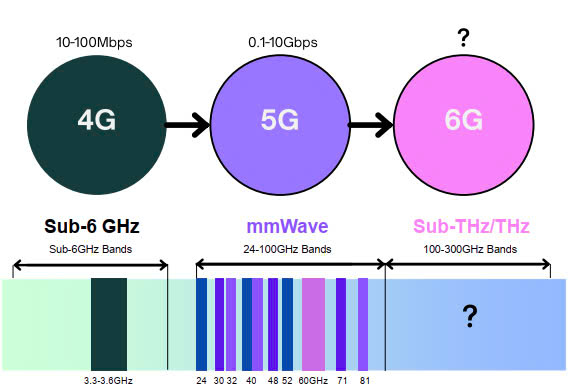
\includegraphics[width=0.6\textwidth]{1.jpg}
    \caption*{Hình 1: Phổ tần số 4G, 5G, 6G \cite{key1} }
    \addcontentsline{lof}{figure}{Hình 1: Phổ tần số 4G, 5G, 6G} 
    \label{fig:model}
\end{figure}
\subsection{1.1 Tại sao chúng ta lại cần nhiều băng thông ?}
Cần nhiều băng thông để đáp ứng tốc độ truyền cao hơn. \\ Theo định luật Shannon: 
\begin{equation}
C = B \log_2(1 + SNR) \tag{1}
\end{equation}
Trong đó: \\
C: Dung lượng kênh truyền (tốc độ dữ liệu tối đa) \\
B: Băng thông (Hz) \\
SNR: Tỷ số tín hiệu trên nhiễu\\

Trong thực tế, SNR thường bị hạn chế bởi nhiễu môi trường (khoảng cách hoặc vật cản), đặc biệt là ở dải tần cao như mmWave và THz. Do đó, để tăng C, ta cần tăng B để truyền dữ liệu nhanh hơn. Với băng thông rộng hơn sẽ cho phép chia sẻ phổ hiệu quả hơn thông qua kĩ thuật beamforming\\

Dù cần nhiều băng thông nhưng việc sử dụng mmWave và THz là không hề đơn giản. Phạm vi truyền ngắn và khả năng xuyên vật cản kém là những hạn chế lớn, đòi hỏi công nghệ tiên tiến như anten, thuật toán học sâu (LSTM) để tối ưu hóa. 



\begin{center}
    \section{Chương 2: Vấn đề xem xét trong truyền sóng}
\end{center}

\subsection{2.1 Mất mát đường dẫn không gian tự do}
Là lượng năng lượng tín hiệu bị mất khi truyền từ anten phát đến anten thu trong môi trường không có vật cản. Phụ thuộc vào khoảng cách và tần số \\
FSPL được mô tả bằng hai công thức chính: \\
\begin{align}
LFSL &= \left( \frac{4\pi R}{\lambda} \right)^2 \tag{2} \\
LFSL_{dB} &= 92.4 + 20\log f + 20\log R \tag{3}
\end{align}
Khi tần số tăng, làm FSPL tăng mạnh. Ta dễ thấy trong hình 2 ở tần số 18GHz, bước sóng khoảng 16,7 mm nhưng ở 100GHz nó chỉ còn 3mm, chứng tỏ mất mát lớn. \\
Lấy ví dụ: Nếu f = 60GHz và R = 10km: \\
20 \log 60 &\approx 35.6 \\
20 \log 10 &= 20 \\
FSPL_{dB} &\approx 92.4 + 35.6 + 20 = 148 \, \text{dB}. \\

Kết quả này khớp với biểu đồ, cho thấy mất mát khoảng 150 dB ở 60GHz và 10km. Khi tần số ở 100GHz, FSPL vượt 180dB ở 100km, gần như không khả thi để truyền xa. Do đó, các hệ thống phải sử dụng nhiều trạm phát sóng nhỏ hoặc công nghệ tái truyền.


\begin{figure}[htbp]
    \centering
    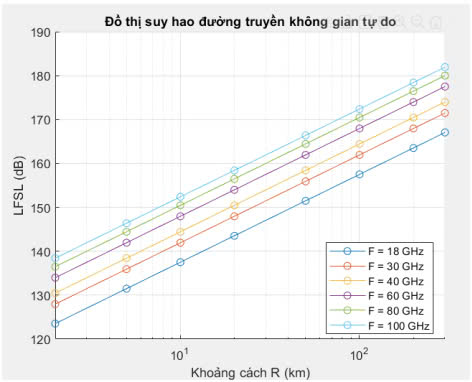
\includegraphics[width=0.55\textwidth]{matmatduongdan.jpg}
    \caption*{Hình 2: Suy giảm trong không gian từ các tần số khác nhau\cite{key2} }
    \addcontentsline{lof}{figure}{Hình 2: Suy giảm trong không gian từ các tần số khác nhau} 
    \label{fig:model}
\end{figure}

Trục y: Mất mát đường dẫn (FSPL) đo bằng dB, dao động từ 120dB đến 190dB\\

Trục x: Khoảng cách truyền (R) đo bằng km, từ 0,1km đến 100km

\subsection{2.2 Cửa sổ khí quyển và Đỉnh suy hao}
Sự hấp thụ khí quyển xảy ra khi sóng điện từ, đặc biệt là mmWave bị các phân tử trong không khí hấp thụ năng lượng, dẫn đến suy hao tín hiệu. \\
Sóng mmWave bị hấp thụ mạnh nhất tại các tần số đặc trưng, gọi là "tần số cộng hưởng". \\
Biểu đồ hình 3 cho thấy, mức độ suy hao thay đổi theo tần số và độ cao. Tại mức nước biển, nơi độ ẩm cao, suy hao có thể lên đến 40dB/km tại các tần số như 22GHz hoặc 193 GHz. Ngược lại, ở độ cao 9150m nơi không khí khô hơn, suy hao giảm đáng kể, chỉ còn vài dB/km tại cùng tần số.
\begin{figure}[htbp]
    \centering
    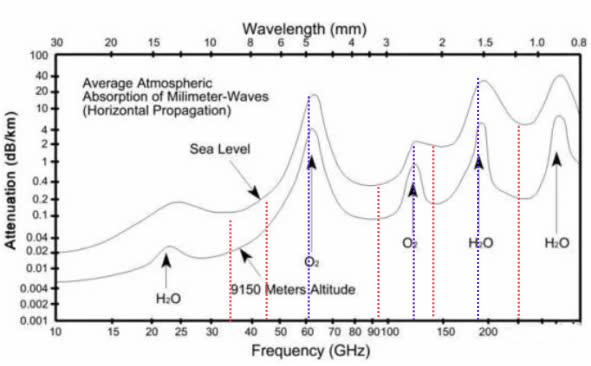
\includegraphics[width=0.5\textwidth]{dinhsuyhao.jpg}
    \caption*{Hình 3: Biểu đồ xu hướng suy giảm khí quyển của mmWave ở các tần số \cite{key2} }
    \addcontentsline{lof}{figure}{Hình 3: Suy giảm trong không gian từ các tần số khác nhau} 
    \label{fig:model}
\end{figure}

\subsection{2.3 Phản xạ khuếch tán}
Phản xạ khuếch tán không chỉ làm giảm năng lượng tín hiệu mà còn dẫn đến hiệu ứng Shadowing. Trong môi trường đô thị, nơi có nhiều vật cản, mmWave dễ bị Shadowing và chỉ hiệu quả trong phạm vi ngắn
\begin{figure}[htbp]
    \centering
    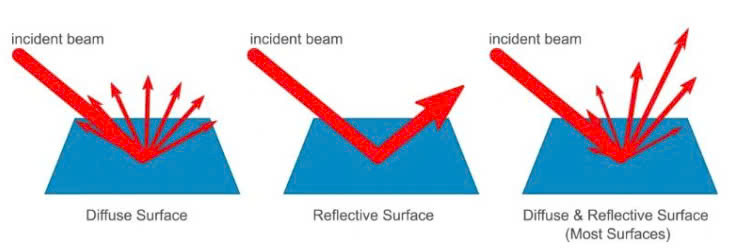
\includegraphics[width=0.6\textwidth]{phanxa.jpg}
    \caption*{Hình 4: Phản xạ khuếch tán và phản xạ gương \cite{key2} }
    \addcontentsline{lof}{figure}{Hình 4: Phản xạ khuếch tán và phản xạ gương} 
    \label{fig:model}
\end{figure} \\
Bề mặt khuếch tán: Sóng đến bị phản xạ theo nhiều hướng khác nhau, năng lượng bị phân tán \\
Bề mặt phản xạ: Sóng đến được phản xạ theo một góc duy nhất, tạo ra phản xạ gương \\
Bề mặt kết hợp: Kết hợp cả 2, năng lượng tín hiệu bị phân tán một phần nhưng vẫn có hướng chính\\

\subsection{2.4 Khả năng xuyên thấu hạn chế}
Là khả năng đi qua các vật liệu như gỗ, kính ... mà không bị suy hao quá nhiều. Sóng mm với tần số (30-300GHz) và bước sóng (1-10mm) 
\begin{figure}[htbp]
    \centering
    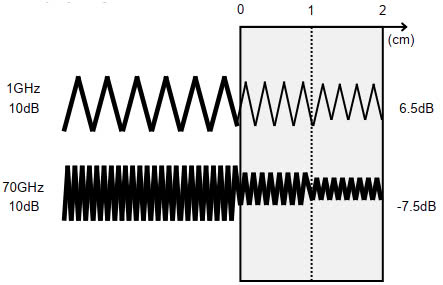
\includegraphics[width=0.4\textwidth]{xuyenthau.jpg}
    \caption*{Hình 5: Suy hao trong một loại vật liệu ở tần số 1GHz và 70GHz \cite{key2} }
    \addcontentsline{lof}{figure}{Hình 5: Suy hao trong một loại vật liệu ở tần số 1GHz và 70GHz } 
    \label{fig:model}
\end{figure}\\
Khi sóng mm đi qua các vật liệu xây dựng phổ biến, tín hiệu mất đi từ 1-6dB cho mỗi cm độ dày. Ở tần số 70GHz (mmWave), suy hao qua từng gạch cao gấp 5 lần so với 1GHz. Điều này xảy ra vì tần số cao hơn làm tăng sự hấp thụ và tán xạ của vật liệu. 

\subsection{2.5 Tiêu thụ năng lượng}
Biểu đồ hình 6 cho thấy mức độ suy hao tăng theo tần số và cường độ mưa: \\
Mưa nhỏ (2.5 mm/h): Ở 100 GHz, suy hao khoảng 10 dB/km, nhưng ở 300 GHz, tăng lên 20 dB/km. \\
Mưa lớn (25 mm/h): Ở 100 GHz, suy hao khoảng 30 dB/km, và ở 300 GHz, lên đến 50 dB/km. \\
Điều này có nghĩa trong điều kiện mưa lớn, tín hiệu mmWave ở tần số cao gần như không thể truyền xa hơn 1km mà không bị suy hao nghiêm trọng
\begin{figure}[htbp]
    \centering
    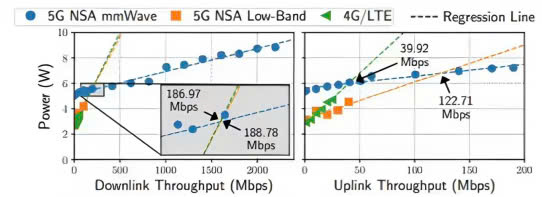
\includegraphics[width=0.5\textwidth]{tieuthua.jpg}
    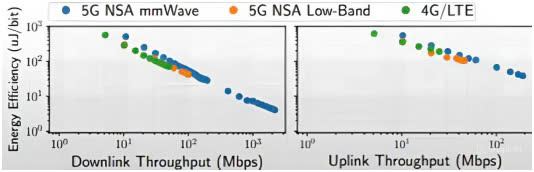
\includegraphics[width=0.44\textwidth]{tieuthub.jpg}
    \caption*{Hình 6: So sánh tiêu thụ năng lượng các loại công nghệ hiện nay \cite{key3} }
    \addcontentsline{lof}{figure}{Hình 6: So sánh tiêu thụ năng lượng các loại công nghệ hiện nay} 
    \label{fig:model}
\end{figure}\\
Ngoài mưa, các điều kiện thời tiết khác cũng ảnh hưởng đến mmWave như: \\
Sương mù gây suy hao nhẹ, thường dưới 1dB/km, nhưng có thể tăng ở tần số rất cao (trên 200GHz). Hơi nước trong không khí tăng hấp thụ, đặc biệt ở các tần số cộng hưởng (22GHz, 183 GHz)\\
Giải pháp: Tăng công suất phát nhưng cũng sẽ làm tăng tiêu thụ năng lượng. Triển khai nhiều trạm phát sóng nhỏ để đảm bảo tín hiệu luôn có đường truyền ngắn, tránh suy hao lớn
\clearpage
\subsection{2.6 Búp sóng hẹp và các búp sóng phụ}
Khi một anten phát tín hiệu, năng lượng không phân bố đều mà tập trung thành các búp sóng. Trong đó, búp sóng chính là khu vực năng lượng tập trung mạnh nhất, thường hẹp \( (30^\circ - 45^\circ) \). Búp sóng phụ là các vùng năng lượng yếu hơn, thường gây nhiễu nếu không được kiểm soát.

\begin{figure}[htbp]
    \centering
    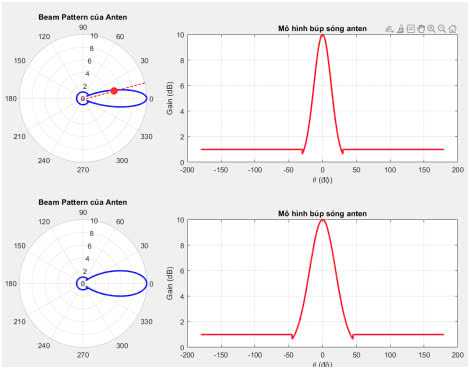
\includegraphics[width=0.5\textwidth]{bupsong.jpg}
    \caption*{Hình 7: Mô hình búp sóng phạm vi \( 30^\circ - 45^\circ \)  \cite{key2} }
    \addcontentsline{lof}{figure}{Hình 7: Mô hình búp sóng phạm vi \( 30^\circ - 45^\circ \) } 
    \label{fig:model}
\end{figure}\\
\textbf{Tại sao không mở rộng góc búp sóng chính ?}\\
Nếu mở rộng góc búp sóng chính, năng lượng sẽ phân tán, làm giảm độ lợi cũng như dễ bị nhiễu từ môi trường \\
Ví dụ ở tần số 60GHz, một anten với búp sóng chính \( 30^\circ \) có thể đạt độ lợi 20-30dB, trong khi mở rộng lên \( 90^\circ \) sẽ giảm độ lợi xuống dưới 10dB, làm suy yếu tín hiệu\\
Công thức (4) mô tả anten theo góc {\theta} \\
\begin{center}
\begin{equation}
G(\theta) = 
\begin{cases} 
G_m 10^{-\frac{3}{10} \left(\frac{20\theta}{\omega}\right)^2}, & |\theta| \leq \frac{\theta_m}{2}, \\
G_s, & \frac{\theta_m}{2} \leq |\theta| \leq \pi,
\end{cases} \tag{4}
\end{equation}
\end{center}\\
Trong đó: \\
\begin{itemize}
    \item Half-power beamwidth: \( \omega \)
    \item Phạm vi búp sóng chính: \( Q_m \)
    \item Độ lợi cực đại: \( G_m \)
    \item Độ lợi trung bình búp sóng phụ: \( G_s \)
\end{itemize}

\begin{center}
    \section{Chương 3: Vật liệu chế tạo}
\end{center}
Trong lĩnh vực công nghệ mmWave - THz, việc lựa chọn vật liệu chế tạo linh kiện đóng vai trò quan trọng để đảm bảo hiệu suất cao, đặc biệt trong các thiết bị như anten, bộ khuếch đại công suất, mạch tích hợp ...
\subsection{3.1 Vật liệu chế tạo mmWave}
Yêu cầu đối với vật liệu mmWave phải cần các yếu tố: \\
Độ linh động electron cao để đảm bảo tín hiệu truyền nhanh\\ Cần chịu được điện áp lớn mà không bị hỏng, do công suất phát tín hiệu cao
\begin{figure}[htbp]
    \centering
    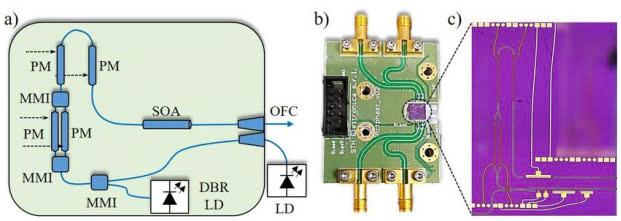
\includegraphics[width=0.6\textwidth]{inp.jpg}
    \caption*{Hình 8: Indium Phosphide \cite{key5} }
    \addcontentsline{lof}{figure}{Hình 8: Indium Phosphide} 
    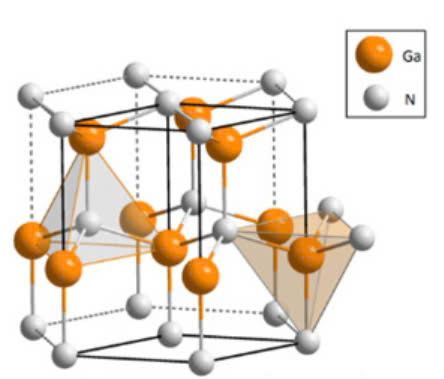
\includegraphics[width=0.35\textwidth]{GaN2.jpg}
    \caption*{Hình 9: Gallium Nitride   }
    \addcontentsline{lof}{figure}{Hình 9: Gallium Nitride } 
    \label{fig:model}
\end{figure}

\begin{table}[h]
    \centering
    \caption{Bảng 1: So sánh đặc tính của Silicon (Si), Gallium Arsenide (GaAs), Indium Phosphide (InP), và Gallium Nitride (GaN)}
     \addcontentsline{lot}{table}{Bảng 1: So sánh đặc tính của Silicon (Si), Gallium Arsenide (GaAs), Indium Phosphide (InP), và Gallium Nitride (GaN)} 
    \begin{tabular}{lcccc}
        \toprule
        \textbf{Đặc tính} & \textbf{Si} & \textbf{GaAs} & \textbf{InP} & \textbf{GaN} \\
        \midrule
        Độ linh động electron (cm²/V·s) & 1400 & 2000 & 5400 & 1500 \\
        Tần số hoạt động (GHz) & <100 & 30-100 & <300 & 30-100 \\
        Điện áp đánh thủng (V) & 10-20 & 20-30 & 20-40 & 50-100 \\
        Độ dẫn nhiệt (W/m·K) & 150 & 50 & 70 & 200 \\
        Chi phí sản xuất & Thấp & Trung bình & Cao & Trung bình-Cao \\
        \bottomrule
    \end{tabular}
    \label{tab:material_comparison}
\end{table} GaN: Độ bền, công suất cao, ứng dụng trong radar ô tô, quân sự. InP: Các ứng dụng tần số cao, quang điện tử, vệ tinh. Si: Dành cho các thiết bị tiêu dùng nhờ chi phí thấp

\subsection{3.2 Vật liệu chế tạo THz}
Dải tần THz(0,1-10THz) đang trở thành trung tâm của các công nghệ mới, từ viễn thông 6G đến cảm biến y học và an ninh. Trong số các vật liệu được nghiên cứu như Carbon Nanotubes (CNTs); Liquid Crytals (LCs) thì Graphene nổi bật nhờ tính linh động electron, khả năng hoạt động tần số cao. 
\begin{figure}[htbp]
    \centering
    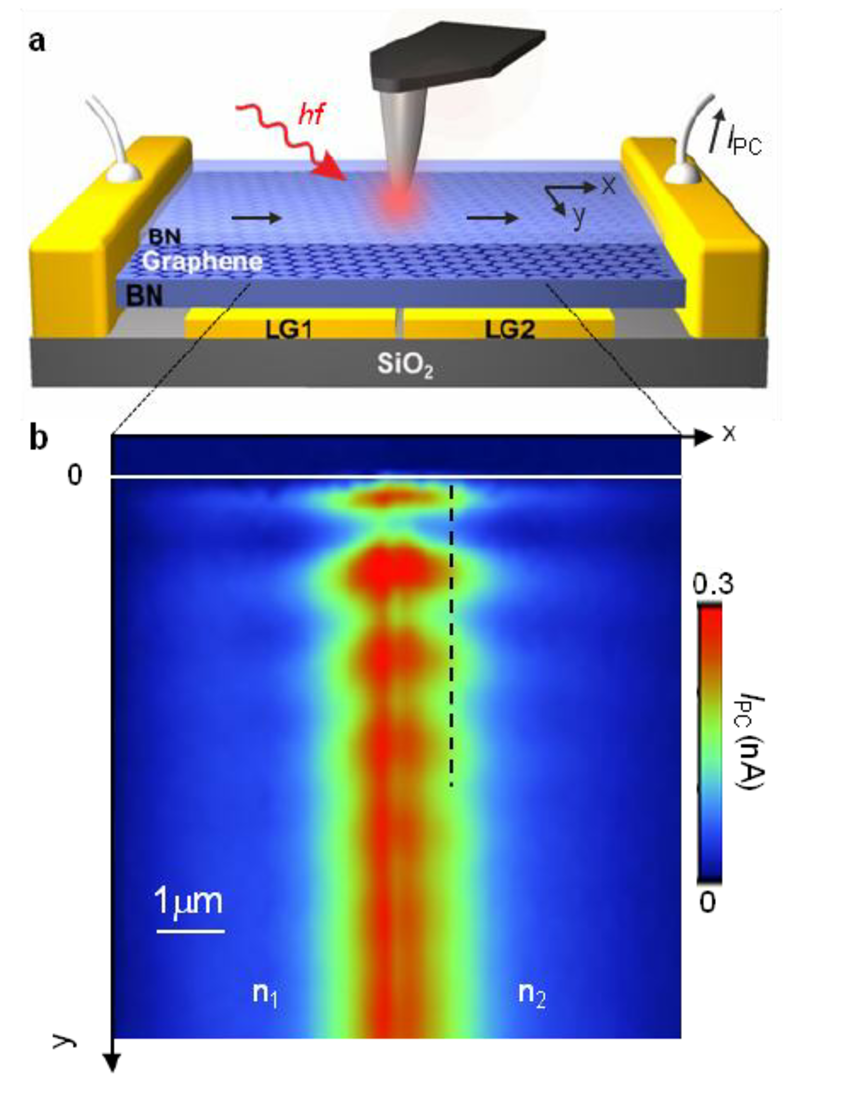
\includegraphics[width=0.7\textwidth]{Graphene.png}
    \caption*{Hình 10: Graphene \cite{key4} }
    \addcontentsline{lof}{figure}{Hình 10: Graphene} 
    \label{fig:model}
\end{figure} \\
Graphene là một vật liệu hai chiều (2D) gồm các lớp carbon nguyên tử được sắp xếp theo cấu trúc "tổ ong". Với độ dày chỉ một nguyên tử, Graphene có:

 \item Độ linh động electron lên đến 200,000 \( \text{cm}^2 \)/V.s, vượt xa Silicon 1400  \( \text{cm}^2 \)/V.s và Indium Phosphide 5400 \( \text{cm}^2 \)/V.s

 \item Độ dẫn điện vượt trội nhờ cấu trúc tinh thể hoàn hảo, Graphene cho phép truyền tín hiệu với tổn thất thấp

\begin{center}
    \section{Chương 4: Công nghệ cốt lõi mmWave}
\end{center}
\subsection{4.1 Thu phát tín hiệu số, tương tự}
Analog Tx (Trạm phát tương tự): Bao gồm DAC (Digital to Analog Converter); LPF (Low Pass Filter); Mixer; RFFE (RF Front End); PS (Phase Shifter) \\ 

Analog Rx (Trạm thu tương tự): Bao gồm RFFE; Mixer, LNA (Low Noise Amplifier); PS; ADC \\

Digital Tx (Trạm phát số): Tương tự Analog Tx, nhưng sử dụng nhiều DAC và Mixer cho từng anten, tăng độ linh hoạt \\

Digital Rx (Trạm thu số): Tương tự Analog Rx, nhưng sử dụng nhiều ADC và Mixer, cho phép xử lí tín hiệu số chi tiết hơn
\begin{figure}[htbp]
    \centering
    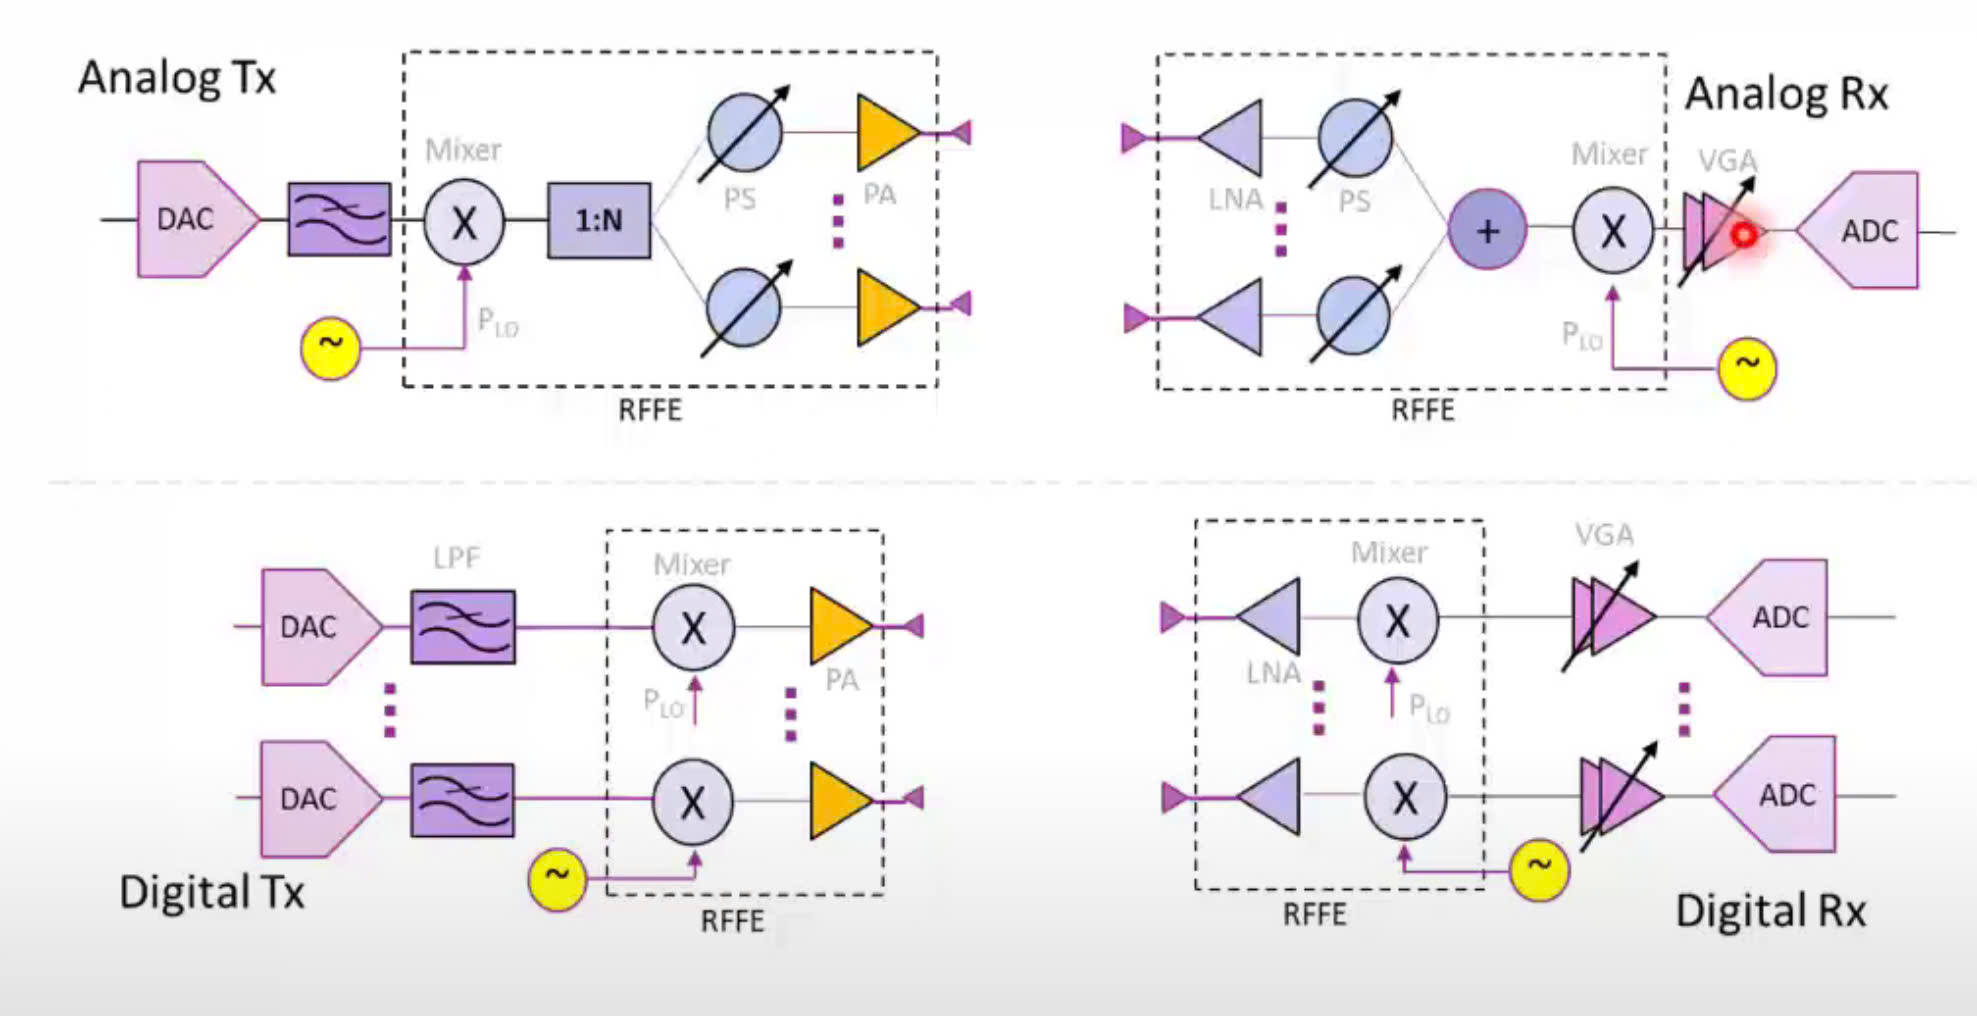
\includegraphics[width=0.7\textwidth]{sodothuphatsotuongtu.jpg}
    \caption*{Hình 11: Sơ đồ thu phát tín hiệu số và tương tự  \cite{key8} }
    \addcontentsline{lof}{figure}{Hình 11: Sơ đồ thu phát tín hiệu số và tương tự} 
    \label{fig:model}
\end{figure} \\
\textbf{Nguyên lí hoạt động:} \\

Analog Tx: Sóng từ DAC được chuyển đổi sang analog qua LPF, trộn tần số bằng Mixer, điều chỉnh pha bằng PS trước khi phát qua RFFE; là quá trình đơn giản, giảm chi phí phần cứng \\

Analog Rx: Tín hiệu nhận được qua RFFE được khuếch đại LNA, trộn tần số, điều chỉnh pha và chuyển sang số bằng ADC, hiệu suất phụ thuộc vào chất lượng PS \\

Digital Tx: Mỗi anten có DAC và Mixer riêng, cho phép xử lí tín hiệu số chi tiết hơn trước khi phát. \\

Digital Rx: Mỗi anten có ADC và Mixer, xử lí tín hiệu số sau khi thu, tăng độ chính xác

\subsection{4.2 Analog - Digital - Hybrid Beamforming}
Analog beamforming là phương pháp truyền thống, sử dụng PS (Phase Shifters) để điều chỉnh pha tín hiệu ở tầng RF, tạo ra một chùm sóng duy nhất 
\begin{align}
\theta = \arcsin\left(\frac{\lambda \Delta \phi}{2\pi d}\right) \tag{5}
\end{align}

\begin{itemize}
    \item \(\lambda\): Bước sóng.
    \item \(\Delta \phi\): Chênh lệch pha giữa hai anten.
    \item \(d\): Khoảng cách giữa các anten.
\end{itemize}

Digital beamforming vượt trội nhờ khả năng xử lí tín hiệu số ở tầng baseband. Mỗi anten có một chuỗi RF riêng (gồm DAC/ADC và Mixer), cho phép điều chỉnh pha và biên độ tín hiệu một cách độc lập 
\begin{align}
\mathbf{y} = \mathbf{H} \mathbf{W} \mathbf{x} + \mathbf{n} \tag{6}
\end{align}
\begin{itemize}
    \item \(\mathbf{W}\): Ma trận tiền mã hóa (điều chỉnh pha và biên độ).
    \item \(\mathbf{x}\): Tín hiệu gốc.
    \item \(\mathbf{y}\): Tín hiệu nhận được.
    \item \(\mathbf{n}\): Nhiễu.
    \item \(\mathbf{H}\): Ma trận kênh.
\end{itemize}

Hybrid beamforming kết hợp ưu điểm của analog và digital, sử dụng một số lượng nhỏ chuỗi RF (DAC/ADC) ở tầng baseband và nhiều PS ở tầng RF. Tín hiệu được xử lí số để tạo ra một số chùm sóng, sau đó phân chia và điều chỉnh pha qua PS trước khi phát qua anten
\begin{align}
\mathbf{y} = \mathbf{H} (\mathbf{W}_{\text{RF}} \mathbf{W}_{\text{BB}}) \mathbf{x} + \mathbf{n} \tag{7}
\end{align}
\begin{itemize}
    \item \(\mathbf{W}_{\text{BB}}\): Ma trận tiền mã hóa ở tầng baseband.
    \item \(\mathbf{W}_{\text{RF}}\): Ma trận pha ở tầng RF (điều chỉnh qua Phase Shifters - PS).
\end{itemize}

\begin{figure}[htbp]
    \centering
    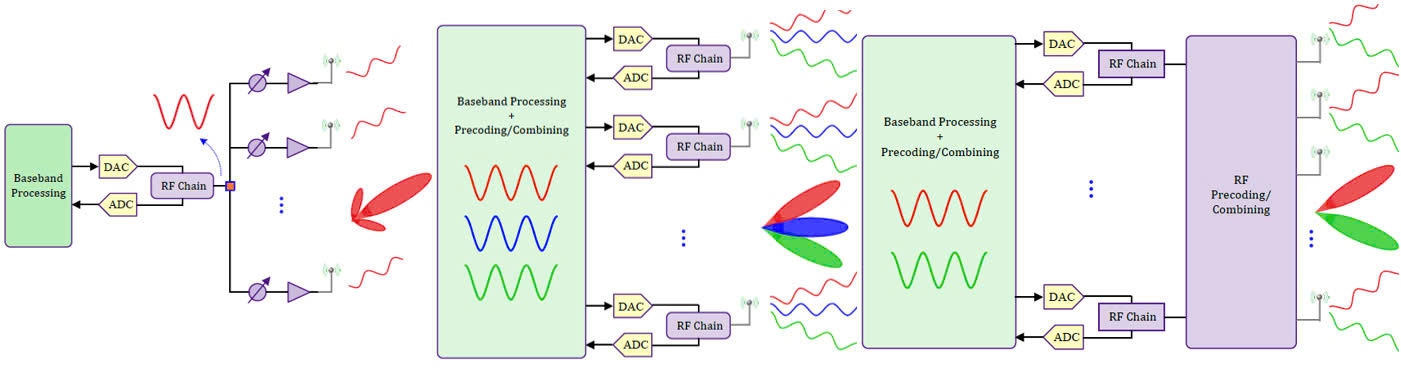
\includegraphics[width=0.73\textwidth]{hybrid.jpg}
    \caption*{Hình 12: Analog - Digital - Hybrid Beamforming  \cite{key8} }
    \addcontentsline{lof}{figure}{Hình 12: Analog - Digital - Hybrid Beamforming } 
    \label{fig:model}
\end{figure}


\clearpage
\subsection{4.3 Mô hình RF Front End}
RF Front End là phần giao tiếp anten và hệ thống xử lí tín hiệu số. Nó xử lí tín hiệu RF (Radio Frequency) trước khi chuyển đổi sang tín hiệu số Rx hoặc sau khi chuyển đổi từ tín hiệu số sang RF (TX)
\begin{figure}[htbp]
    \centering
    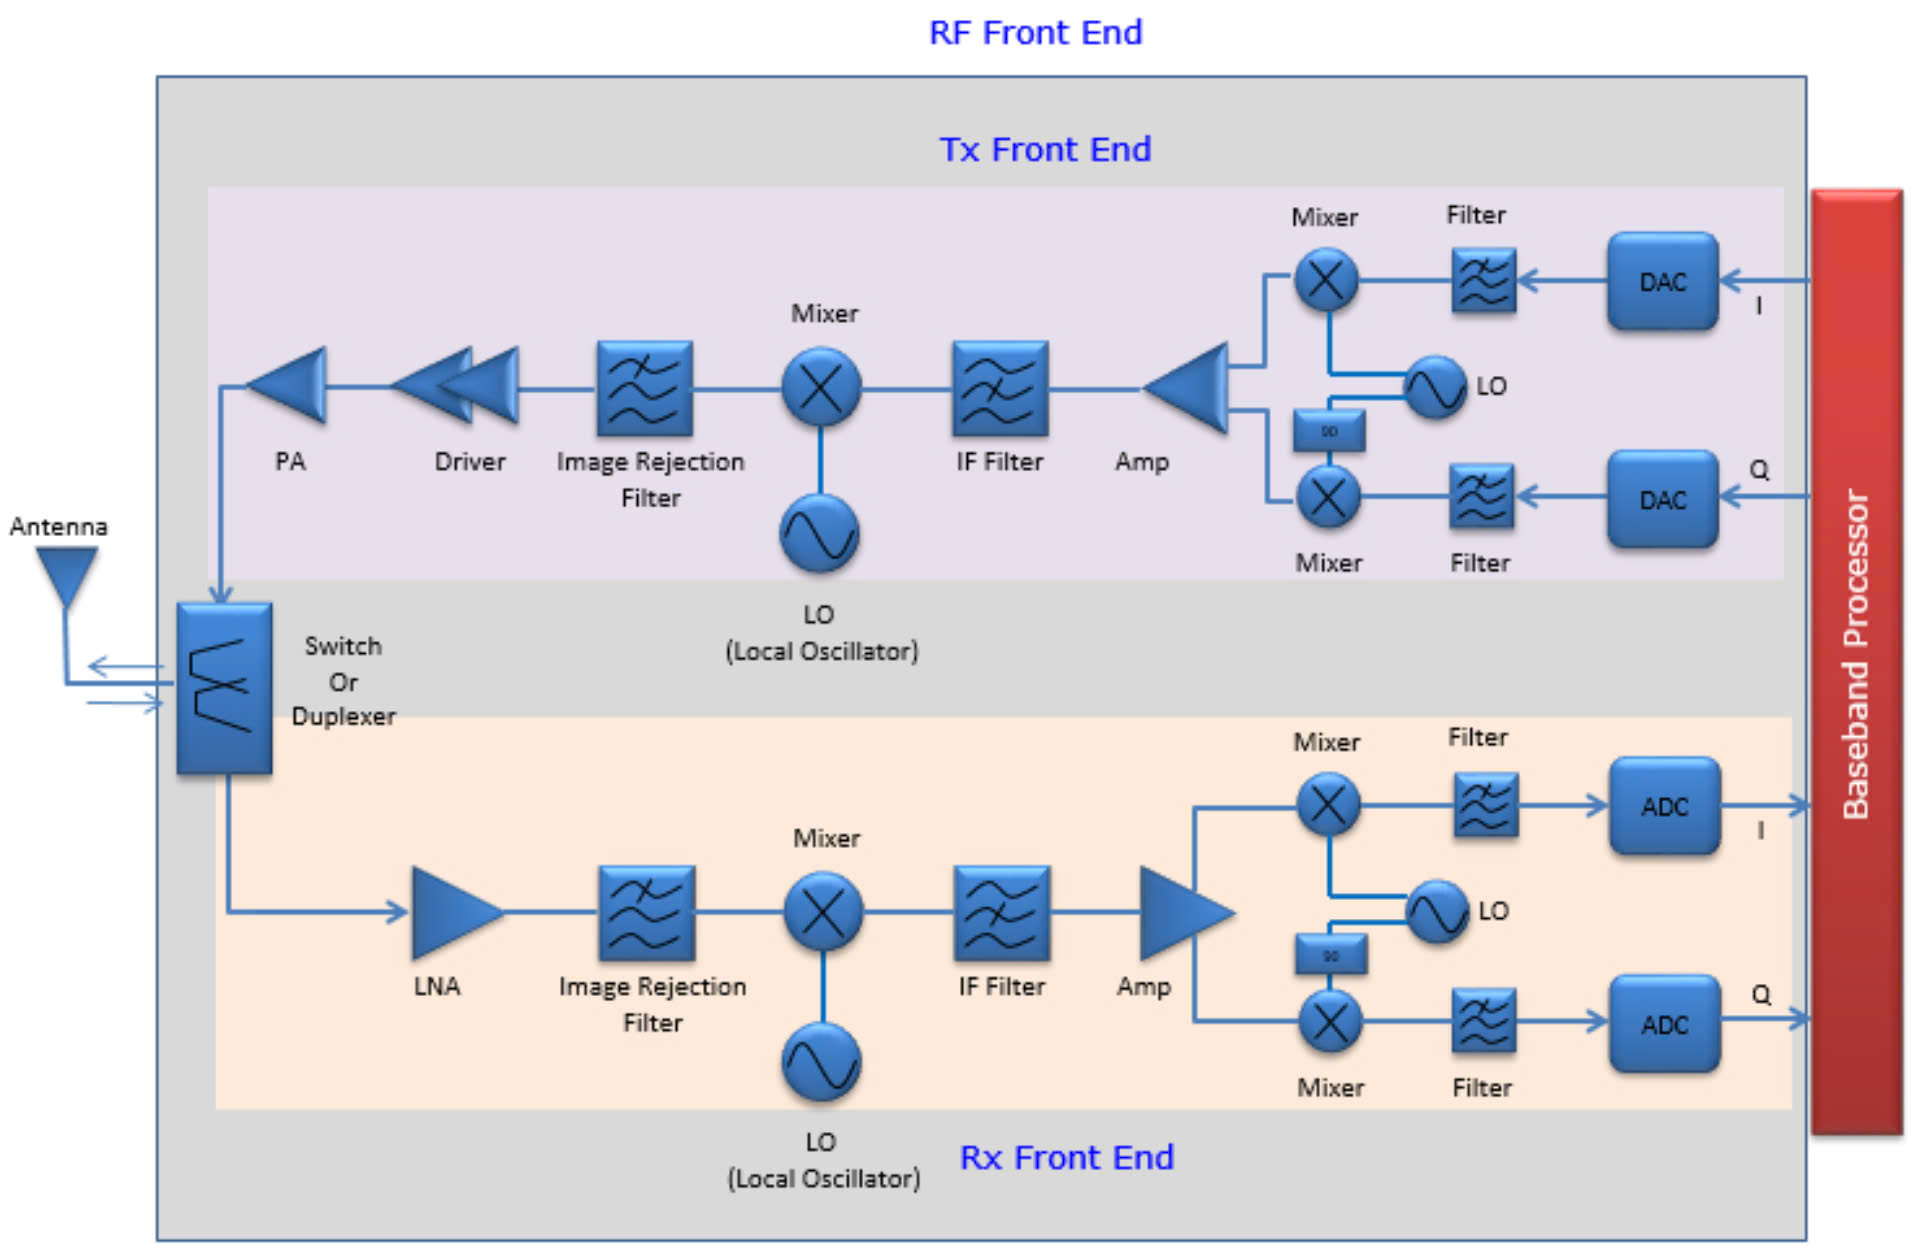
\includegraphics[width=0.84\textwidth]{RF.jpg}
    \caption*{Hình 13: Sơ đồ RF Front End \cite{key8} }
    \addcontentsline{lof}{figure}{Hình 13: Sơ đồ RF Front End } 
    \label{fig:model}
\end{figure}
\begin{itemize}
\item Duplexer/Switch: Chuyển đổi giữa Tx và Rx, đảm bảo tín hiệu không bị chồng lấn
\item Low Noise Amplifier (LNA): Khuếch đại tín hiệu ở RX, giảm nhiễu để tăng SNR
\item Power Amplifier (PA): Khuếch đại tín hiệu ở Tx, đảm bảo tín hiệu đủ mạnh để vượt qua suy hao mmWave
\item Mixer: Chuyển đổi tần số (lên tần số ở Tx, xuống tần số ở Rx) bằng cách trộn tín hiệu với Local Oscillator (LO)
\item Filter: Lọc nhiễu (BPF loại bỏ nhiễu ngoài dải, LPF lọc nhiễu tần số cao)
\item Phase Shifter (PS): Điều chỉnh pha tín hiệu, hỗ trợ beamforming
\end{itemize}
Ở Tx, tín hiệu số từ DAC được nâng tần số qua Mixer, khuếch đại qua PA, điều chỉnh pha (nếu có beamforming), và phát qua anten. \\
Ở Rx, tín hiệu mmWave từ anten được khuếch đại qua LNA, hạ tần số qua Mixer, lọc nhiễu, và chuyển đổi thành số qua ADC.
\begin{center}
   \section{Chương 5: Công nghệ cốt lõi THz} 
\end{center}
\subsection{5.1 Tổng quan về hệ thống THz transmission}
Sơ đồ hình 13 mô tả hệ thống đo lường, trong đó chùm tia THz được tạo ra, truyền qua mẫu và được phát hiện để thu thập thông tin về tính chất quang học của mẫu
\begin{figure}[htbp]
    \centering
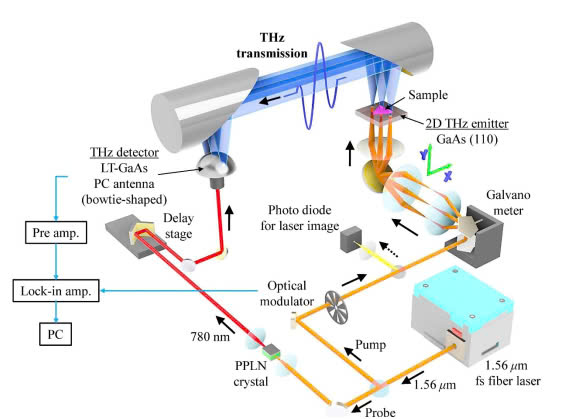
\includegraphics[width=0.67\textwidth]{THz5.jpg}
    \caption*{Hình 14: Hệ thống THz Transmission\cite{key6} } \\

    \addcontentsline{lof}{figure}{Hình 14: THz } 
    \label{fig:model}
\end{figure} \\
\textbf{Nguyên lí hoạt động:}
\begin{itemize}
\item Laser fs (1.56 um) được chuyển đổi thành ánh sáng 780 nm qua PPLN crystal và optical modulator
\item Sóng THz truyền qua mẫu, bị biến đổi bởi các đặc tính hấp thụ, khúc xạ, hoặc tán xạ của mẫu, mang theo thông tin quang học
\item Ánh sáng dò (1.56 μm) kích thích LT-GaAs PC antenna hình bow-tie, nơi tín hiệu THz được chuyển đổi thành dòng điện quang dẫn
\item Delay stage điều chỉnh thời gian trễ giữa ánh sáng bơm và dò, cho phép tái tạo dạng sóng THz trong miền thời gian
\item Tín hiệu được khuếch đại bởi pre-amplifier và xử lý bởi lock-in amplifier để cải thiện tỷ số tín hiệu-nhiễu (SNR)
\item Photodiode và galvanometer hỗ trợ đồng bộ hóa laser và quét chùm tia qua mẫu, có thể được sử dụng để tạo hình ảnh THz 2D
\end{itemize}


\subsection{5.2 Sơ đồ THz s-SNOM}
Sơ đồ hình 14 mô tả hệ thống gần trường THz hoạt động theo chế độ tự đồng pha, sử dụng nguồn phát THz QCL và bộ dò THz QWP. Hệ thống được thiết kế để giảm thiểu tổn thất năng lượng THz và tối ưu hiệu suất ở tần số 4.2 THz
\begin{figure}[htbp]
    \centering
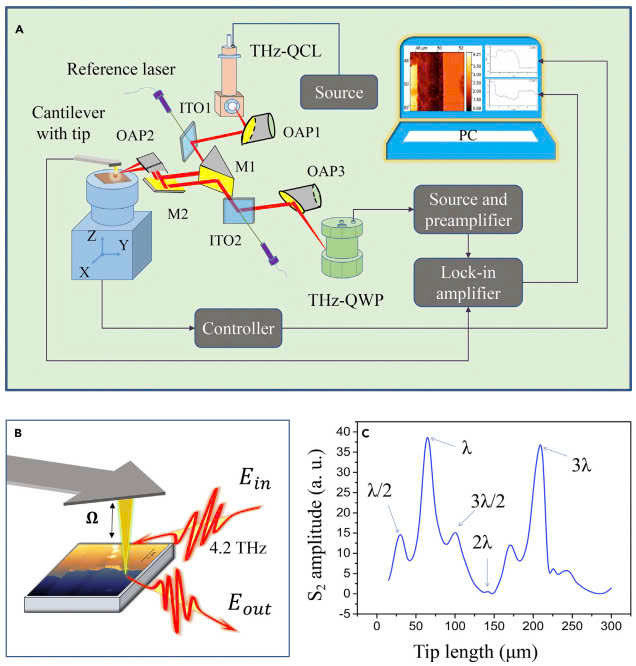
\includegraphics[width=0.67\textwidth]{QCL2.jpg}
    \caption*{Hình 15: a: Hệ thống QCL công suất cao và QWP nhanh; b: Biểu diễn khái niệm gần tán xạ đầu; c Biên độ mô phỏng của tín hiệu S2 với các chiều dài khác nhau\cite{key5} } \\

    \addcontentsline{lof}{figure}{Hình 15: a: Hệ thống QCL công suất cao và QWP nhanh } 
    \label{fig:model}
\end{figure} \\
\textbf{Nguyên lí hoạt động:}
\begin{itemize}
\item THz QCL phát ra chùm tia 4.2 THz chiếu lên mẫu tạo ra trường không bức xạ, chứa thông tin tần số không gian cao
\item Gương parabol lệch trục (OAP1, OAP2, OAP3) và gương ITO/Phẳng (M1,M2) dẫn hướng và tập trung chùm tia THz vào đầu dò AFM và mẫu, sau đó thu thập tín hiệu tán xạ đến QWP
\item Đầu dò AFM kim loại ở tần số cộng hưởng 13kHz dao động ở chế độ tapping để tăng cường và điều chế tín hiệu
\item THz QWP phát hiện tín hiệu tán xạ với thời gian đáp ứng picosecond

\end{itemize}


\subsection{5.3 Công thức trường điện tán xạ THz}
\begin{equation}
E_s = \alpha^{\text{eff}} (1 + \gamma)^2 E_i  \tag{8}
\label{eq:scattered_field}
\end{equation}
trong đó:
\begin{itemize}
    \item \( \gamma \): Hệ số phản xạ xa trường của bề mặt mẫu.
    \item \( \alpha^{\text{eff}} \): Độ phân cực hiệu dụng của liên kết đầu dò-mẫu.
    \item \( E_i \): Cường độ trường điện tới.
\end{itemize}

\begin{equation}
\alpha^{\text{eff}} = \frac{\alpha (1 + \beta)}{1 - \frac{\alpha \beta}{16 \pi (a + d)^3}} \tag{9}\label{eq:effective_polarizability}
\end{equation}
trong đó:
\begin{itemize}
    \item \( \alpha \): Độ phân cực của đầu dò.
    \item \( \beta \): Hàm đáp ứng điện môi của mẫu.
    \item \( a \): Bán kính của đầu dò.
    \item \( d \): Khoảng cách giữa đầu dò và mẫu.
\end{itemize} 

\begin{equation}
\alpha = 4 \pi a^3 \frac{\varepsilon_t - 1}{\varepsilon_t + 2} \tag{10}\label{eq:polarizability}
\end{equation}

\begin{equation}
\beta = \frac{\varepsilon_s - 1}{\varepsilon_s + 1} \tag{11}\label{eq:dielectric_response}
\end{equation}
trong đó:
\begin{itemize}
    \item \( \varepsilon_t \): Hằng số điện môi của đầu dò.
    \item \( \varepsilon_s \): Hằng số điện môi của mẫu.
\end{itemize}


\clearpage
\begin{center}
    \section{Chương 6: Thuật toán cho Beamforming}
\end{center}

\subsection{6.1 Sơ đồ LSTM (Long short Term Memory)}
Giao thông thông minh đòi hỏi các giải pháp tích hợp dữ liệu đa phương thức từ RADAR, LIDAR, GPS và Camera để tối ưu hóa truyền thông và dự đoán hành vi. Vậy cần phải sử dụng mô hình LSTM để xử lí dữ liệu thời gian liên tục, đặc biệt giải quyết vấn đề gradient biến mất trong mạng nơ-ron tuần hoàn (RNN). 
\begin{figure}[htbp]
    \centering
    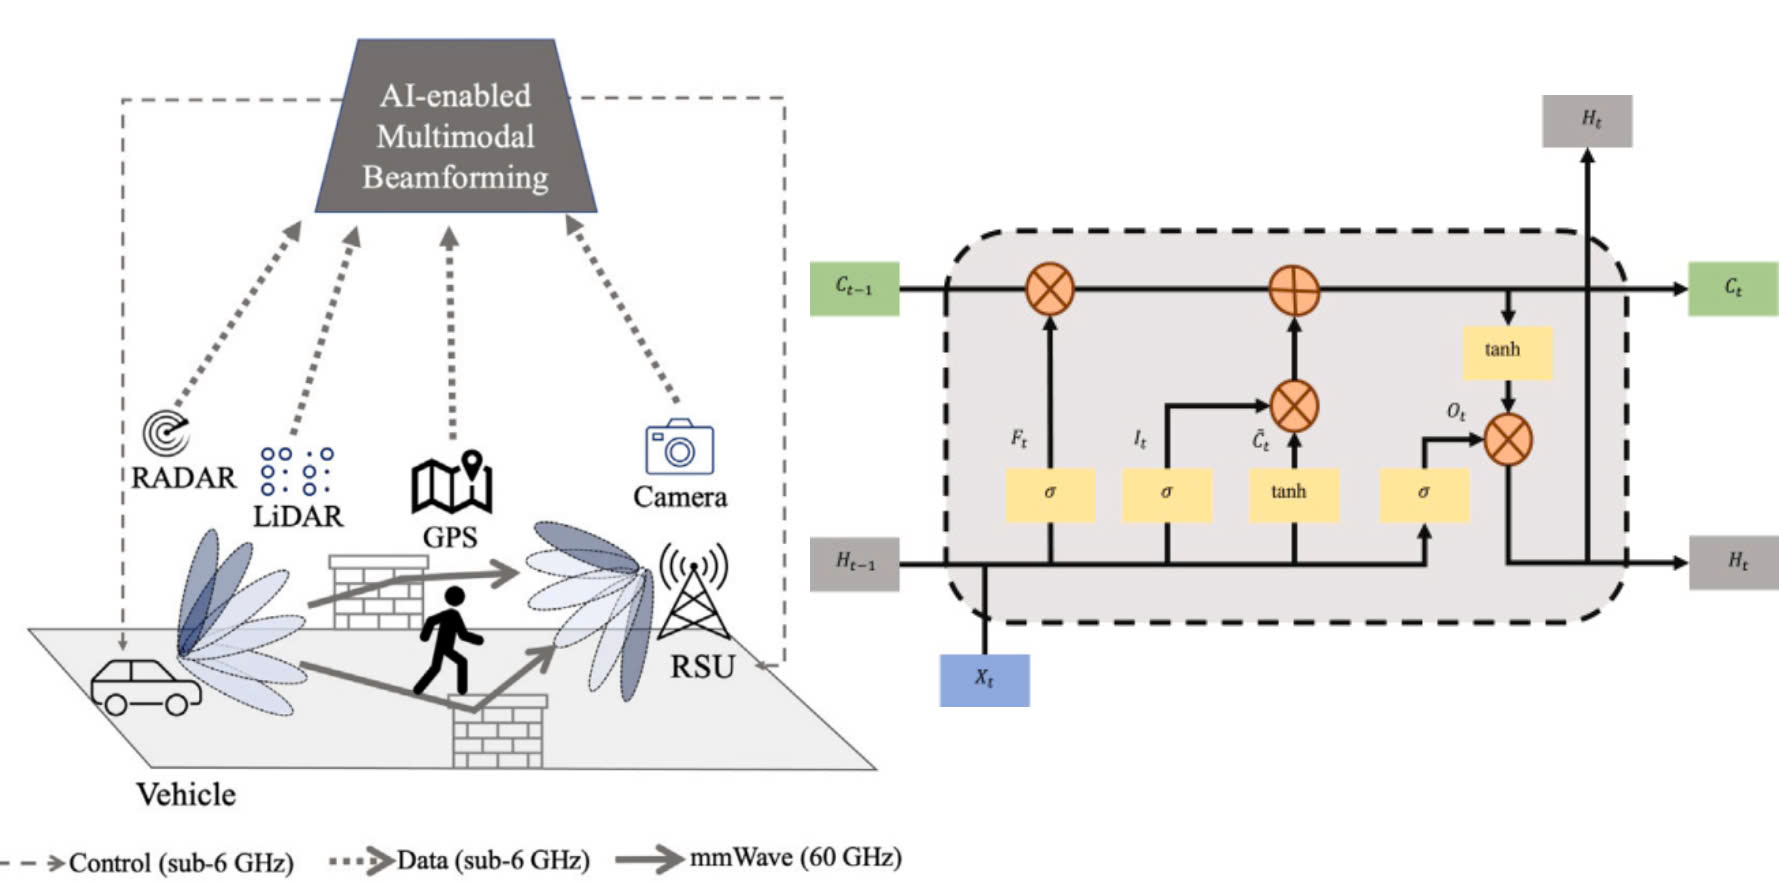
\includegraphics[width=0.9\textwidth]{LSTM.JPG}
    \caption*{Hình 16: Sử dụng mô hình LSTM học sâu }
    \addcontentsline{lof}{figure}{Hình 16: Sử dụng mô hình LSTM học sâu} 
    \label{fig:model}
\end{figure}\\
Sơ đồ hình 15 minh họa quy trình từ thu thập dữ liệu, trạng thái ẩn và bộ nhớ (x_t),(h_t),(C_t) \\

Theo tài liệu, vấn đề gradient biến mất xảy ra khi gradient suy giảm theo cấp số nhân qua nhiều lớp, làm mất khả năng học phụ thuộc dài hạn. LSTM khắc phục hạn chế của RNN bằng các cổng (forget, input, output) và trạng thái bộ nhớ

\begin{figure}[htbp]
    \centering
    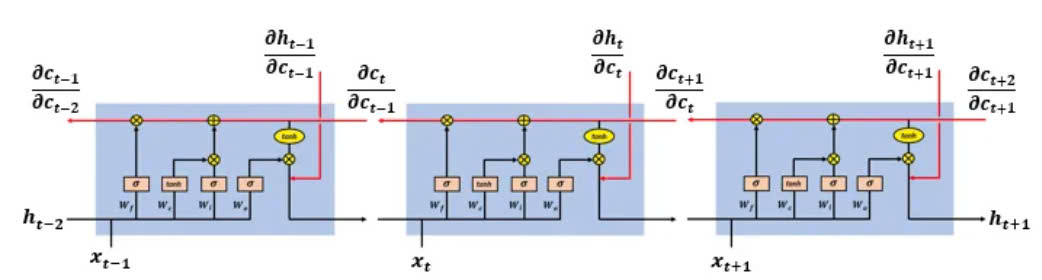
\includegraphics[width=1\textwidth]{LSTM5.jpg}
    \caption*{Hình 17: Mô hình LSTM tổng quát\cite{key10} }
    \addcontentsline{lof}{figure}{Hình 17: Mô hình LSTM tổng quát} 
    \label{fig:model}
\end{figure}

\clearpage
\subsection{6.2 LSTM hoạt động thế nào ?}
LSTM hoạt động dựa trên một đơn vị (cell) tại mỗi bước thời gian t, gồm ba cổng chính \\
Trạng thái bộ nhớ \( {C}_t \) để lưu trữ thông tin qua các bước thời gian
\begin{equation}
C_t = f_t \cdot C_{t-1} + i_t \cdot \tilde{C}_t \tag{12}\label{eq:cell_state_update}
\end{equation}
\( {C}_t \) được cập nhật bằng cách kết hợp thông tin cũ  \( {C}_t-1 \) và thông tin mới \( \tilde{C}_t \) \\
Phép cộng thay vì nhân liên tục như trong RNN giúp gradient không bị giảm mạnh
\begin{figure}[htbp]
    \centering
    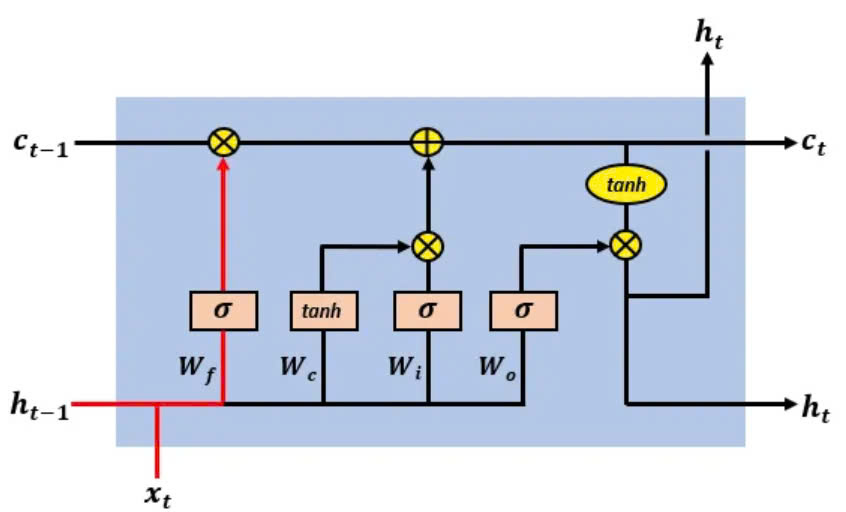
\includegraphics[width=0.5\textwidth]{LSTM2.jpg}
    \caption*{Hình 17: Giai đoạn 1: Cổng quên (Forget)\cite{key10} }
    \addcontentsline{lof}{figure}{Hình 18: Giai đoạn 1: Cổng quên (Forget)} 
    \label{fig:model}
\end{figure}\\
Vai trò: Quyết định thông tin nào từ trạng thái bộ nhớ trước đó \( {C}_t-1 \) sẽ được giữ lại hoặc loại bỏ


\begin{equation}
f_t = \sigma(W_f \cdot [h_{t-1}, x_t] + b_f) \label{eq:input_gate} \tag{13}
\end{equation}
\begin{itemize}
    \item \( f_t \): Giá trị cổng đầu vào tại thời điểm \( t \), nằm trong khoảng \([0, 1]\).
    \item \( W_f \): Ma trận trọng số của cổng đầu vào.
    \item \( b_f \): Vector bias của cổng đầu vào.
    \item \( [h_t-1, x_t] \): Phép nối
\end{itemize}


\clearpage
\begin{figure}[htbp]
    \centering
    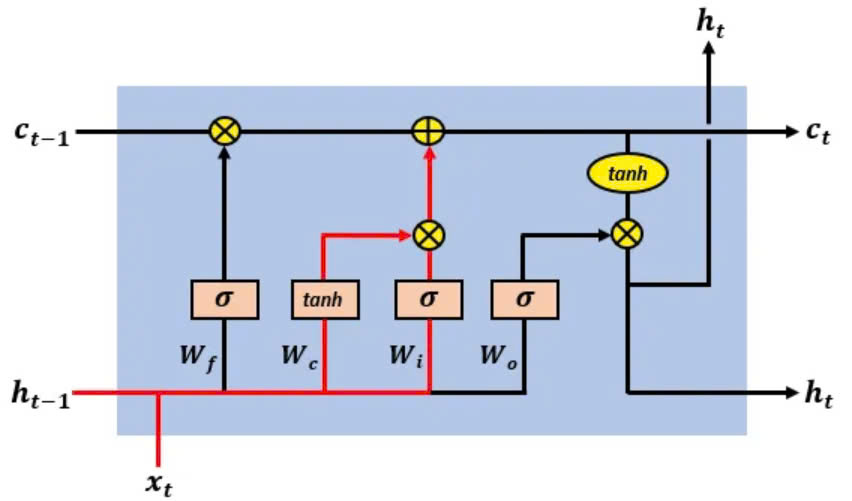
\includegraphics[width=0.5\textwidth]{LSTM3.jpg}
    \caption*{Hình 19: Giai đoạn 2: Cập nhật thông tin mới \cite{key10} }
    \addcontentsline{lof}{figure}{Hình 18: Giai đoạn 2: Cập nhật thông tin mới} 
    \label{fig:model}
\end{figure}


\begin{equation}
\tilde{C}_t = \tanh(W_c \cdot [h_{t-1}, x_t] + b_c)  \tag{14}\label{eq:candidate_cell_state}
\end{equation}

\begin{itemize}
    \item \( \tanh \): Hàm hyperbolic tangent, \( \tanh(x) = \frac{e^x - e^{-x}}{e^x + e^{-x}} \).
    \item \( W_c \): Ma trận trọng số của ứng viên trạng thái.
    \item \( b_c \): Vector bias của ứng viên trạng thái.
\end{itemize}

\begin{figure}[htbp]
    \centering
    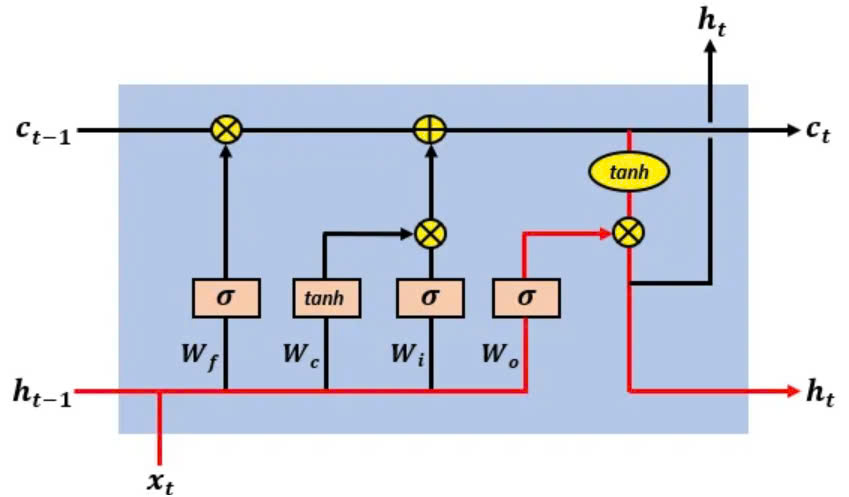
\includegraphics[width=0.6\textwidth]{LSTM4.jpg}
    \caption*{Hình 20: Giai đoạn 3: Cổng đầu ra\cite{key10} }
    \addcontentsline{lof}{figure}{Hình 19: Giai đoạn 3: Cổng đầu ra} 
    \label{fig:model}
\end{figure}\\

\begin{equation}
o_t = \sigma(W_o \cdot [h_{t-1}, x_t] + b_o) \tag{15}\label{eq:output_gate}
\end{equation}

\begin{equation}
h_t = o_t \cdot \tanh(C_t) \tag{16}\label{eq:hidden_state}
\end{equation}
\begin{itemize}
    \item \( o_t \): Giá trị cổng đầu ra tại thời điểm \( t \), nằm trong khoảng \([0, 1]\).
    \item \( W_o \): Ma trận trọng số của cổng đầu ra.
    \item \( b_o \): Vector bias của cổng đầu ra.
    \item \( h_t \): Trạng thái ẩn tại thời điểm \( t \), được sử dụng cho dự đoán hoặc truyền sang bước tiếp theo.
\end{itemize}
\begin{center}
    \section{KẾT LUẬN}
\end{center}
Kết luận nghiên cứu
Công nghệ mmWave và THz đang mở ra những triển vọng mới cho lĩnh vực viễn thông và truyền thông không dây, với khả năng cung cấp tốc độ truyền dữ liệu vượt trội và hỗ trợ các ứng dụng tiên tiến như thực tế ảo, y tế từ xa, và giao thông thông minh. Những phân tích trong tài liệu cho thấy mmWave (30-300 GHz) đã được triển khai trong mạng 5G tại nhiều quốc gia, bao gồm Việt Nam, với tốc độ tải xuống ấn tượng như 4,3 Gbps trong thử nghiệm của Qualcomm. \\

Trong khi đó, THz (0,1-10 THz) hứa hẹn tốc độ hàng trăm Gbps, dù vẫn đang trong giai đoạn nghiên cứu.
Tuy nhiên, cả hai công nghệ này đều đối mặt với nhiều thách thức kỹ thuật. Mất mát đường dẫn không gian tự do (FSPL), suy hao khí quyển, phản xạ khuếch tán, khả năng xuyên thấu hạn chế, tiêu thụ năng lượng cao và búp sóng hẹp là những vấn đề nổi bật. Ví dụ, tại 60 GHz, FSPL có thể lên tới 148 dB ở khoảng cách 10 km, khiến việc truyền tín hiệu xa trở nên khó khăn. Các điều kiện thời tiết như mưa hay hơi nước cũng làm tăng suy hao, đặc biệt ở dải tần THz.\\

Để vượt qua những thách thức này, nghiên cứu đã nhấn mạnh vai trò của vật liệu chế tạo và công nghệ cốt lõi. Các vật liệu như Indium Phosphide (InP), Gallium Nitride (GaN) và Graphene mang lại độ linh động electron cao và khả năng hoạt động ở tần số lớn, giúp cải thiện hiệu suất thiết bị. Đồng thời, các công nghệ như beamforming (analog, digital, hybrid) và mô hình RF Front End tối ưu hóa việc truyền tín hiệu, trong khi thuật toán học sâu LSTM hỗ trợ dự đoán và điều chỉnh chùm sóng hiệu quả hơn, đặc biệt trong các ứng dụng giao thông thông minh.\\

Trong bối cảnh Việt Nam đang thúc đẩy chuyển đổi số, việc phát triển và ứng dụng mmWave và THz không chỉ đáp ứng nhu cầu băng thông ngày càng tăng mà còn góp phần vào sự phát triển bền vững. Tuy nhiên, để đưa các công nghệ này từ lý thuyết vào thực tiễn, cần tiếp tục đầu tư nghiên cứu, thử nghiệm và triển khai các giải pháp kỹ thuật tiên tiến.



\clearpage
\begin{center}
    \section{TÀI LIỆU THAM KHẢO}
\end{center}

\printbibliography
\end{document}

